\documentclass{article}
\usepackage{geometry}
\usepackage[utf8]{inputenc}
\usepackage{graphicx}
% package and file page setting for image input
\graphicspath{ {images/} }

%Allows for linking within document and externally
\usepackage{hyperref}
%setup for hyperref colour schemes
\hypersetup{
    colorlinks=true,
    linkcolor=blue,
    filecolor=magenta,      
    urlcolor=cyan,
    pdftitle={Sharelatex Example},
    pdfpagemode=FullScreen,
    }

\usepackage{geometry}
% package for setting page format and size, and setting paragraph indents, paragraph spacing, and line spacing. 
\geometry{a4paper, left=25mm, right=25mm, top=25mm, bottom=25mm}
\setlength{\parindent}{2em}
\setlength{\parskip}{1em}
\renewcommand{\baselinestretch}{1.3}
% for Baseline stretch
% 1 = 1 line spacing in Word 
% 1.3 = 1.5 line spacing in Word 
% 1.5 = double spacing in Word

\usepackage{fancyhdr}
%package to include header and footer information. Only starts from second page with these settings.
\pagestyle{fancy}
\fancyhf{}
\rhead{Proof of Concept - Planning to Publish}
\lhead{S. Goldie - 42611814}
\lfoot{FOAR705 - Digital Humanities}
\rfoot{Page \thepage}




\title{Proof of Concept - Planning to Publish}
\author{Sheriden Goldie}
\date{Session 2, 2019}

\begin{document}

\maketitle

\tableofcontents
%creates a table of contents based on sections and subsections

\pagebreak
%ends text on current page, and moves all following text to the next page.

\section{Introduction}

The GitHub Repository which has all the related files for this project can be found at: \url{https://github.com/MQ-FOAR705/SGoldie_ScrivToTexThesis}

This project walk through is designed to give you the basic understanding of how to use Scrivener to create a .tex compatible file. This file can be manipulated to create a document with professional typesetting, consistently and efficiently. 

This walkthrough assumes a basic level of digital literacy.

\section{Requirements}

Before beginning the project walk through, please ensure you have the following programs installed:

\begin{itemize}
    \item Scrivener - This can be downloaded from \url{https://www.literatureandlatte.com/}
    \item TeXWorks Editor - This can be downloaded from \url{https://www.tug.org/texlive/}
\end{itemize}

Scrivener is a proprietary software, but you can try it for free for 30 non-consecutive days, and this trial version is a complete software download. 

TeXWorks Editor (Also called TexLive) is a free, open-source software that has significant technical support available online through the website listed above, and services like \url{https://tex.stackexchange.com/}.

You will also need to download the scrivener template, scrivener compile settings, and Thesis Formatting Commands files to your computer. Ensure that these files are saved to a location that you can easily navigate to - for example the desktop.


\section{Importing a Scrivener Template}

When you first open Scrivener, you will be prompted to create a project. 

There are many useful templates available through Scrivener, and I encourage you to explore them to gain familiarity with the program in your own time. 

To achieve the purpose of this walk through we will create a project based on the template file I have created, and you will have downloaded to your computer desktop.

This is the window you should see:

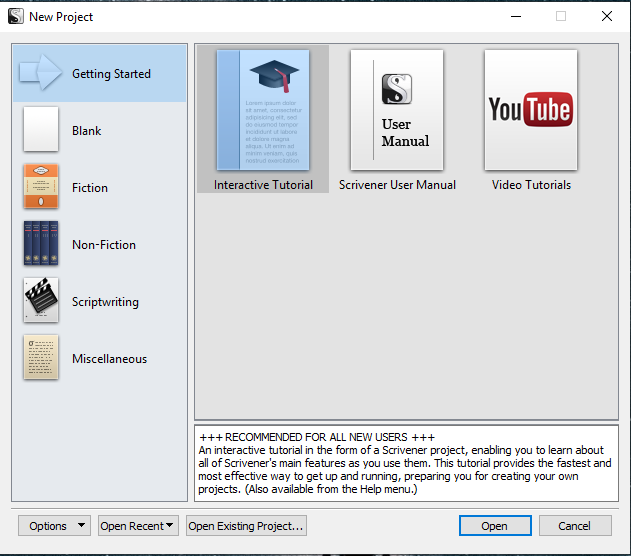
\includegraphics[width=350px]{images/scriv001.PNG}

At the bottom left of the window, there will be an options dropdown menu. 

Select the ``Import templates'' option.

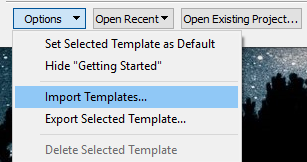
\includegraphics[width=200px]{images/scriv002.PNG}

A folder directory window will open. Navigate to where you saved the Template file to. In this case it is the Desktop.

Select the file and click open.

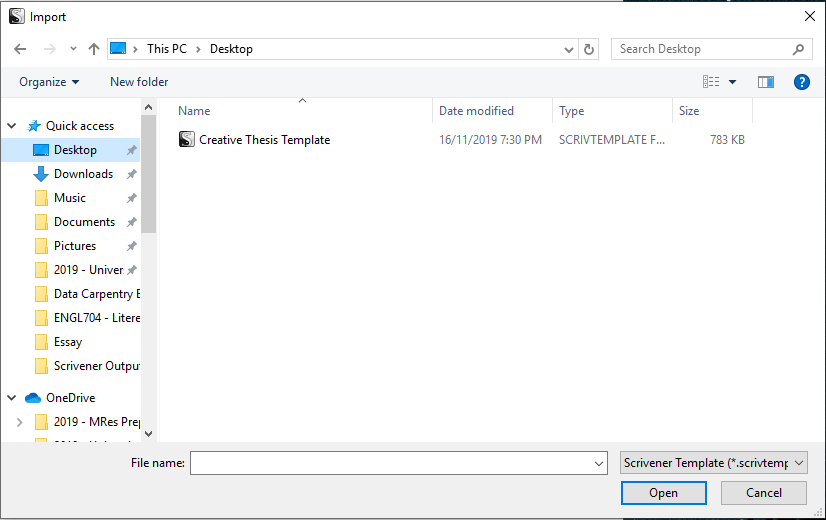
\includegraphics[width=350px]{images/scriv003.PNG}

It will appear as if nothing happens. Close the window and reopen Scrivener.

Now if you select the ``Blank'' category on the left hand side, the ``Creative Thesis Template'' will appear in the space on the right.

Select this template.

Name your project, and select a location that you wish to save the project to.

Then click on ``Create''

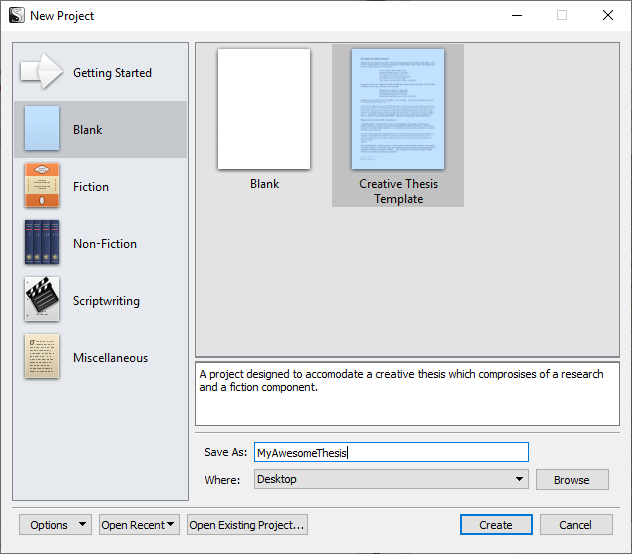
\includegraphics[width=350px]{images/scriv004.PNG}


\section{Using Scrivener}

Scrivener is a large and relatively complex program. It has a lot of uses, and many tools and features that are beneficial. 

I encourage you to refer to the online forums and existing tutorial information for how to get the most out of Scrivener for your own writing project.

Scrivener is, at its most basic, a text storing tool. You can type text into it, and it will save it for you, for later use. 

It features some formatting options, but that is not it's primary use.

I will review some of the key functionalities below

\subsection{The Binder}

The Binder occupies the left side of the window. You can choose to have it visible or not by clicking on the binder button at the top right of the window.

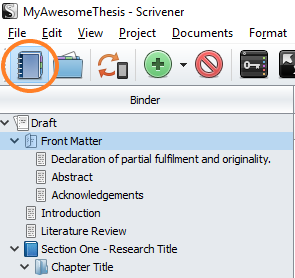
\includegraphics[width=200px]{images/scriv005.PNG}

The Binder is one way Scrivener visualises the organisation of your project. 

The three most basic parts of the Binder, are ``Draft,'' ``Research,'' and ``Trash''

These parts cannot be changed, but you can manipulate their contents as much as you like. 

In the bottom right, there are buttons for creating new documents and new folders. Or you can use ctrl+n for a new document, or ctrl+shift+n for a new folder. Whichever section is highlighted in blue is the section that your new document or folder will appear under, but you can click and drag to move things around if you wish. 

\subsection{Index Cards}

Every item in The Binder will have an Index card. This appears in the Corkboard view, and the Inspector, and imitate the look of an old index card - a small lined piece of heavy cardstock, used to store small discrete pieces of data. Library catalogues would employ index cards extensively.

In Scrivener you can use the Index card to hold whatever information you choose. It is most effective when it isn't more than a  few sentences.

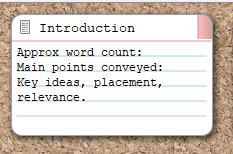
\includegraphics[width=200px]{images/scriv008.PNG}

When a section has multiple documents within it, like section one and two in the above screenshot, the index card will appear to have another behind it. If you select that section and view it in the corkboard view, it will have it's own set of index cards for those subsections. 

\subsection{The Corkboard}

At the top centre of the window, there are three ways to view the selected section of your project. 

The corkboard view, shows the index cards in a grid layout. 

You can drag and drop to move sections to reorder them if you wish. 

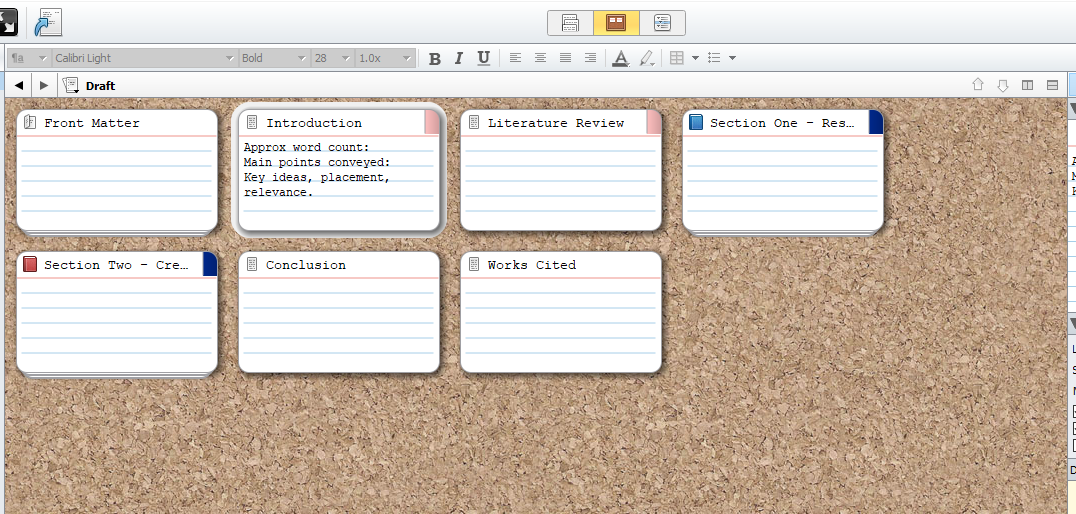
\includegraphics[width=350px]{images/scriv006.PNG}

\subsection{Outline}

In the same way - an outline view can be selected, and shows the same information in a text oriented way. 

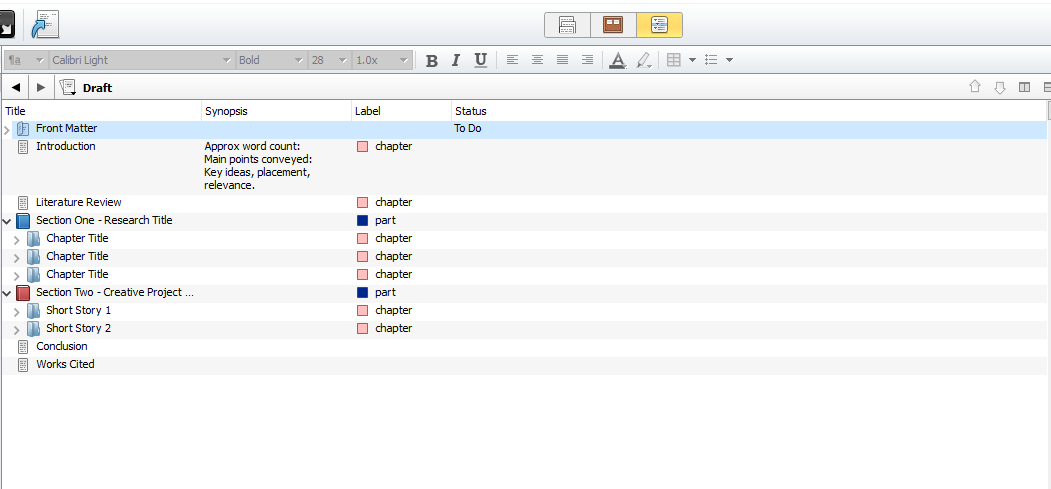
\includegraphics[width=350px]{images/scriv007.PNG}

\subsection{Inspector}

The Inspector panel can be viewed by clicking the blue i icon at the top right of the window. 

In this panel, the information from the index card is displayed, as well as many other things. 

There is also a place to keep notes regarding this document specifically.   

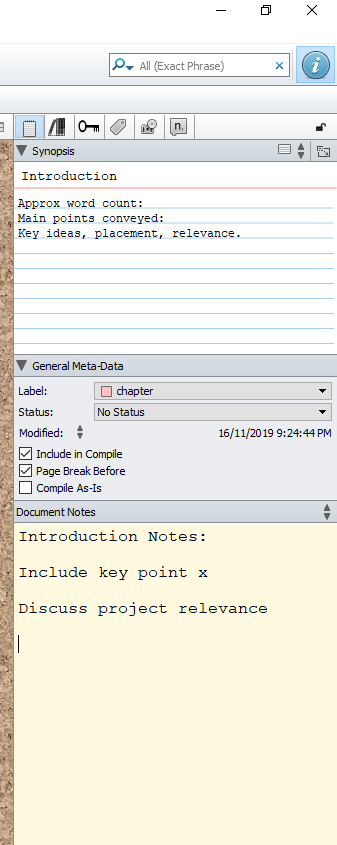
\includegraphics[width=130px]{images/scriv009.PNG}

The document notes section has a drop down that can be switched to general project notes as well.

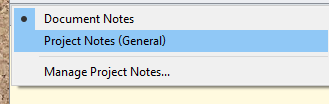
\includegraphics[width=200px]{images/scriv010.PNG}

\section{Importing Compile Settings to Scrivener}

When you have completed a draft - or anytime throughout the process you wish - you will want to compile your draft. 

Compiling will combine all the documents in your draft according to the formatting guidelines you set, for the output you select. 

I have saved a set of compile settings for this project. 

To import these click on compile (The button that looks like a document page with a blue arrow):

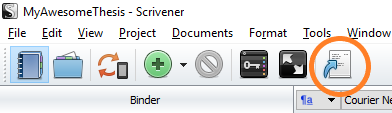
\includegraphics[width=200px]{images/scriv011.PNG}

Click on the ``load preset'' button:

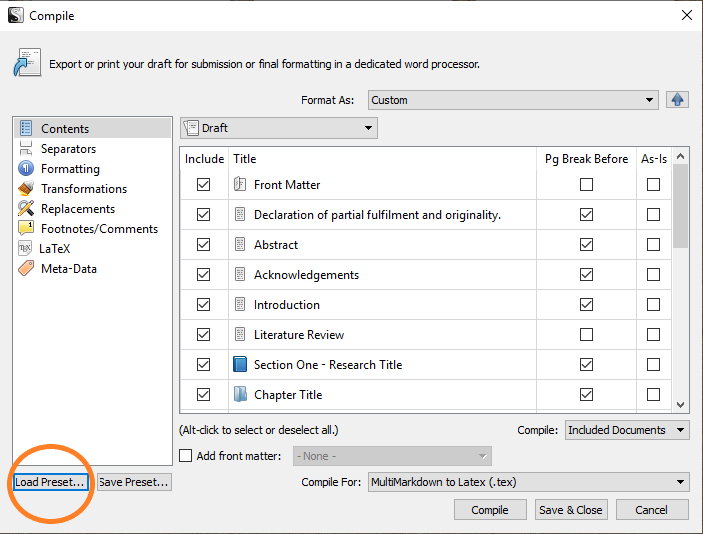
\includegraphics[width=200px]{images/scriv012.PNG}


click on the ``import'' button:

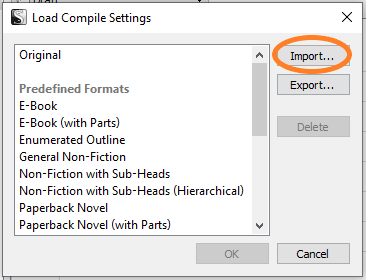
\includegraphics[width=200px]{images/scriv013.PNG}


navigate to the location the that LatexThesis.ini file was saved to - this should be the same place as the temaplate file - so in this case it is the Desktop.

Click on Open:

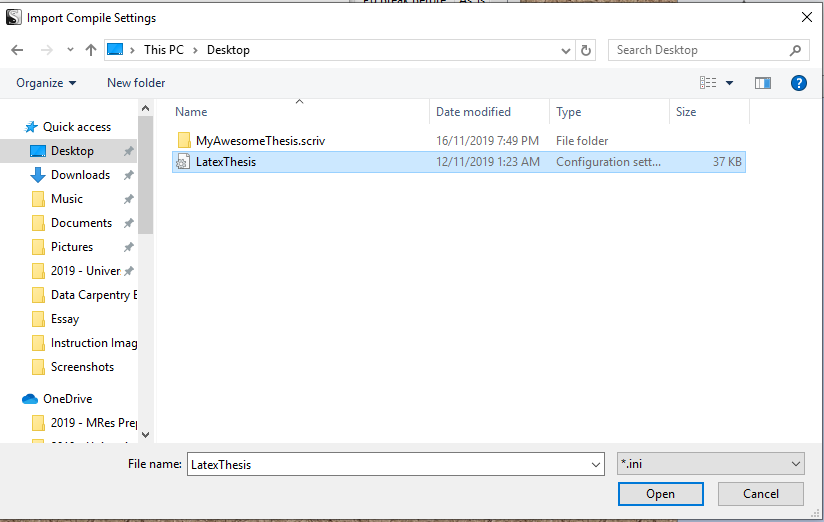
\includegraphics[width=200px]{images/scriv014.PNG}

Then you will appear back at the ``import'' window, and if you scroll down you will see the LatexThesis option under ``My Formats.''

Select this, and click OK.

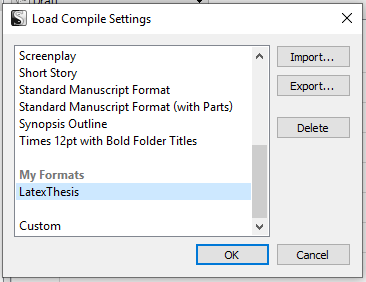
\includegraphics[width=200px]{images/scriv015.PNG}

Now you will be in the main Compile window, with the format set to LatexThesis in the dropdown in the top right of the window. 

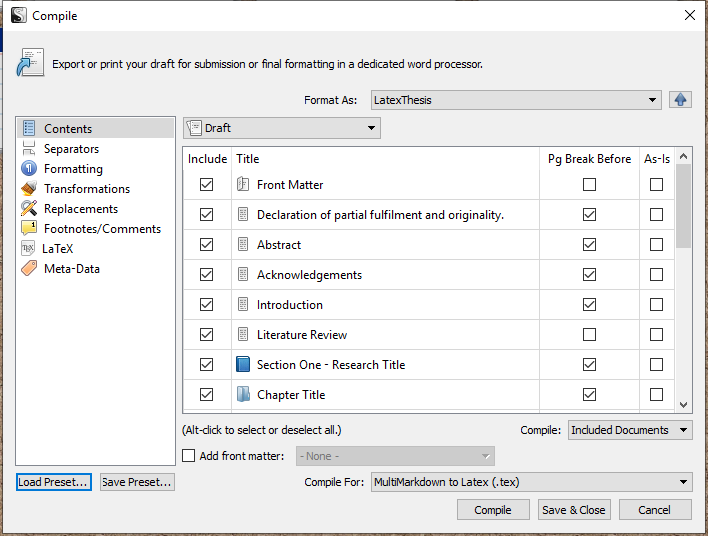
\includegraphics[width=200px]{images/scriv016.PNG}

You can now compile the document.

A window will open to prompt you to decide where you would like the file saved. I have chosen the desktop for this example. Click Save

Note - do not save it within the Scrivener project file. 

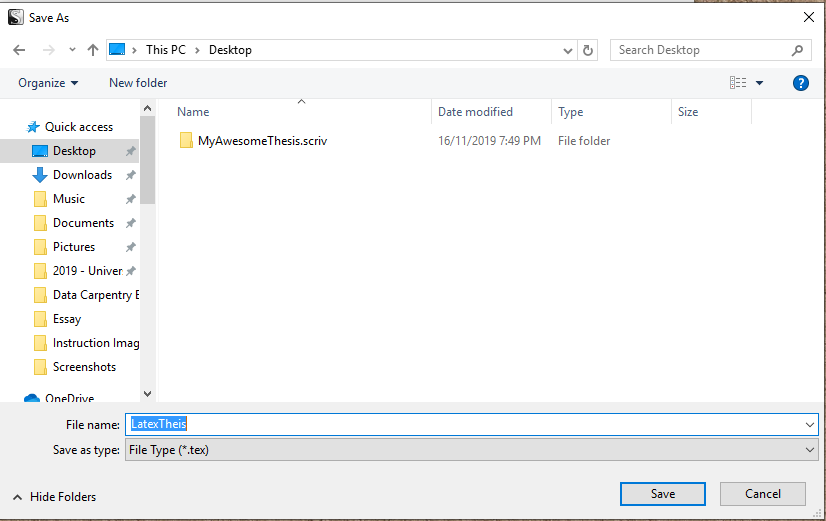
\includegraphics[width=200px]{images/scriv017.PNG}

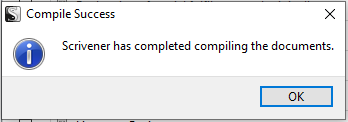
\includegraphics[width=200px]{images/scriv018.PNG}


\section{Compiling a LaTeX file in TexWorks Editor}

To finalise the document in a LaTeX formatted document, you will need to open the file you just compiled in TexWorks Editor. 

If you have already installed TexWorks, the file will open automatically if you double click it from its folder location.

Or you can open TexWorks and open the file from the menu in TexWorks.

The file will look like this:

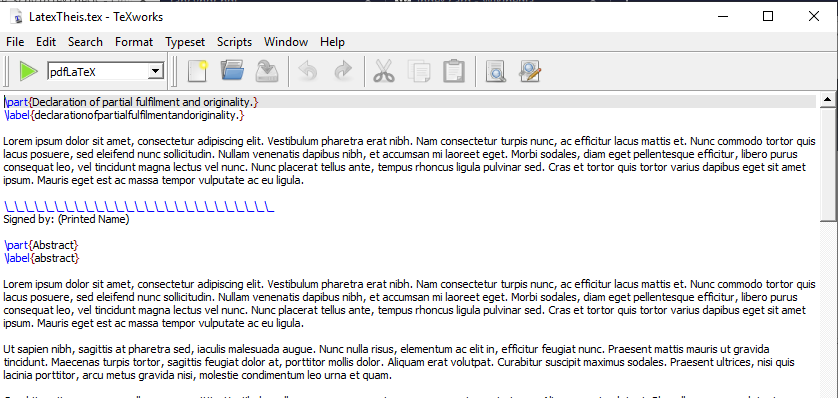
\includegraphics[width=350px]{images/tex001.PNG}

you will also need to open the ThesisFormattingCommands.tex file 

The ThesisFormattingCommands.tex file is divided into sections, with notes on where to include these in your thesis document.

It will look like this:

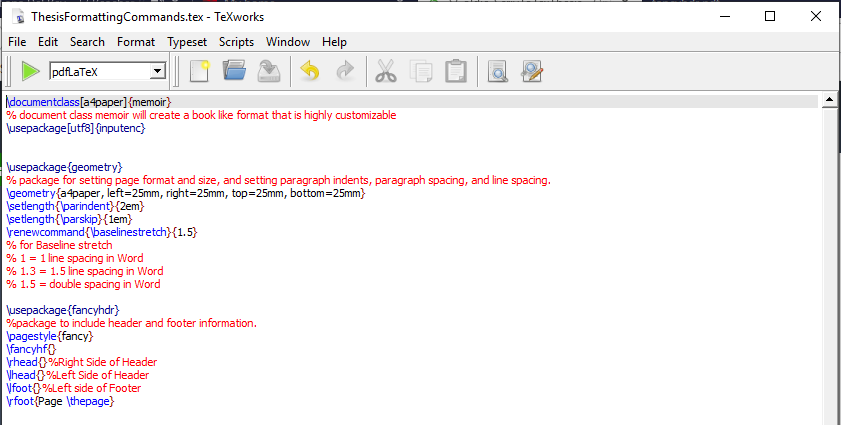
\includegraphics[width=350px]{images/tex002.PNG}

In the ThesisFormattingCommands.tex file there are some sections that you will need to fill in manually. These are highlighted in the document - with notes that begin with a \% symbol. The main title page will require your attention, as will the header and footer information should you wish to include that.


In the exported file from Scrivener, some of the sections are automatically assigned the command 'part', and these will need to be changed to 'chapter*'

Do this for the Declaration, Abstract, Acknowledgement, Introduction, Literature Review, Conclusion, and Works Cited. 

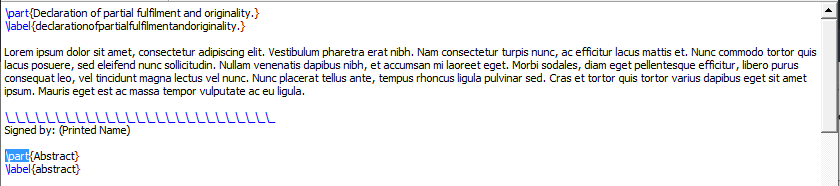
\includegraphics[width=350px]{images/tex003.PNG}

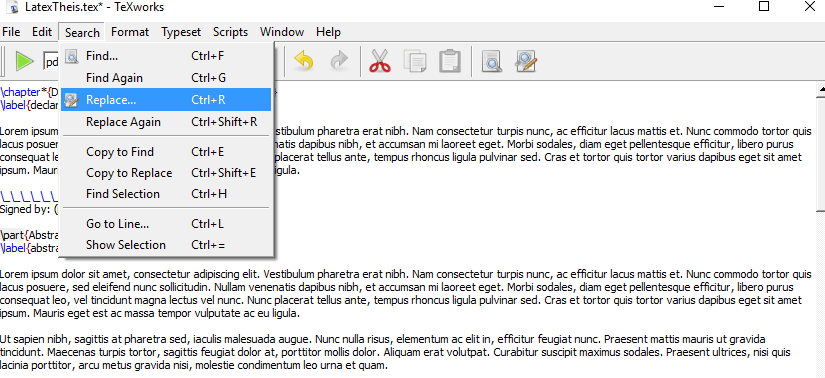
\includegraphics[width=350px]{images/tex004.PNG}

Use the find and replace function to make this quicker if you like - but you will need to check each replace - as we don't want to replace all of them. You can use the ctrl+shift+r to ``replace again'' just make sure your cursor in the document is BEFORE the item you want to replace - not in or on the item. 

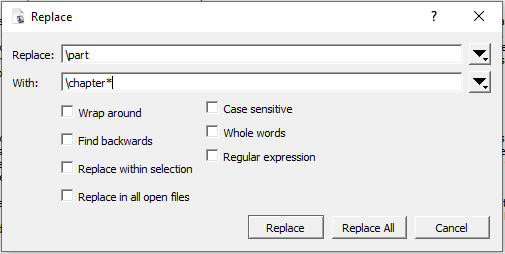
\includegraphics[width=200px]{images/tex005.PNG}

Then you will need to copy sections of the ThesisFormattingCommands.tex into the thesis document. 

Copy the contents up to the first line of \% symbols. Paste this at the the very beginning of the thesis document. 

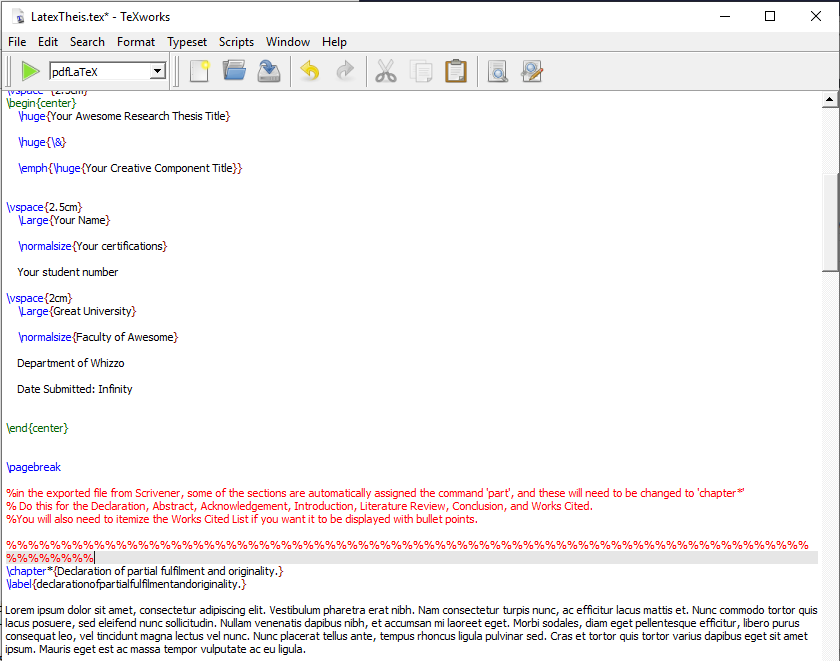
\includegraphics[width=350px]{images/tex006.PNG}

Then copy the next section - between the next lines of \% symbols, and paste this after the Acknowledgements, and before the Introduction. 

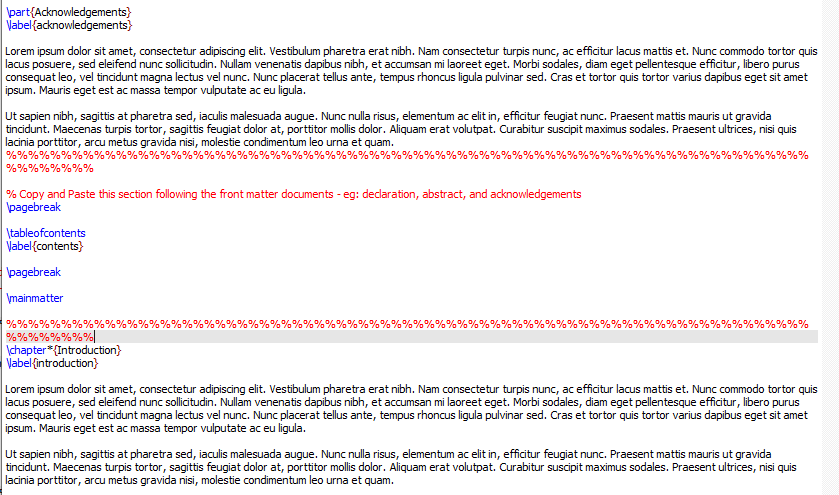
\includegraphics[width=350px]{images/tex007.PNG}

Copy the final section, and paste this at the very end of your thesis document

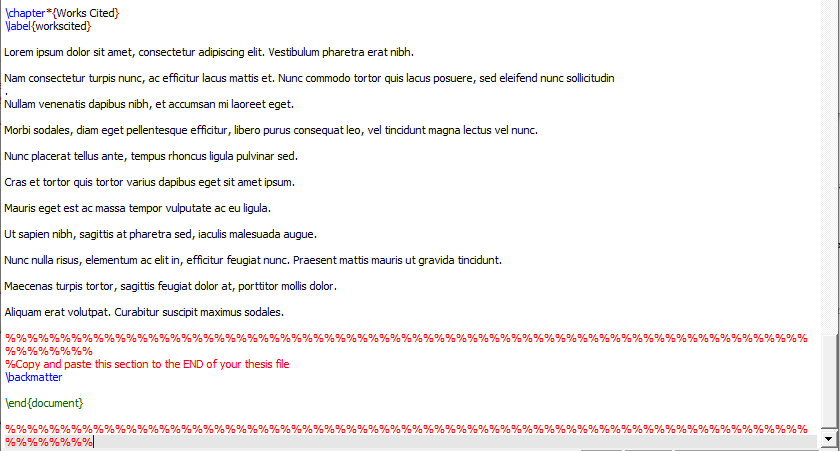
\includegraphics[width=350px]{images/tex008.PNG}

Now you are ready to process this document in TexWork Editor to produce a PDF document.

Click the green play arrow at the top left of the TexWorks window:

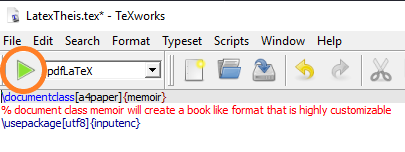
\includegraphics[width=300px]{images/tex009.PNG}


A Processing window will appear in the bottom of the window, and when it is complete a new window will appear showing a rendering of the formatted PDF document.

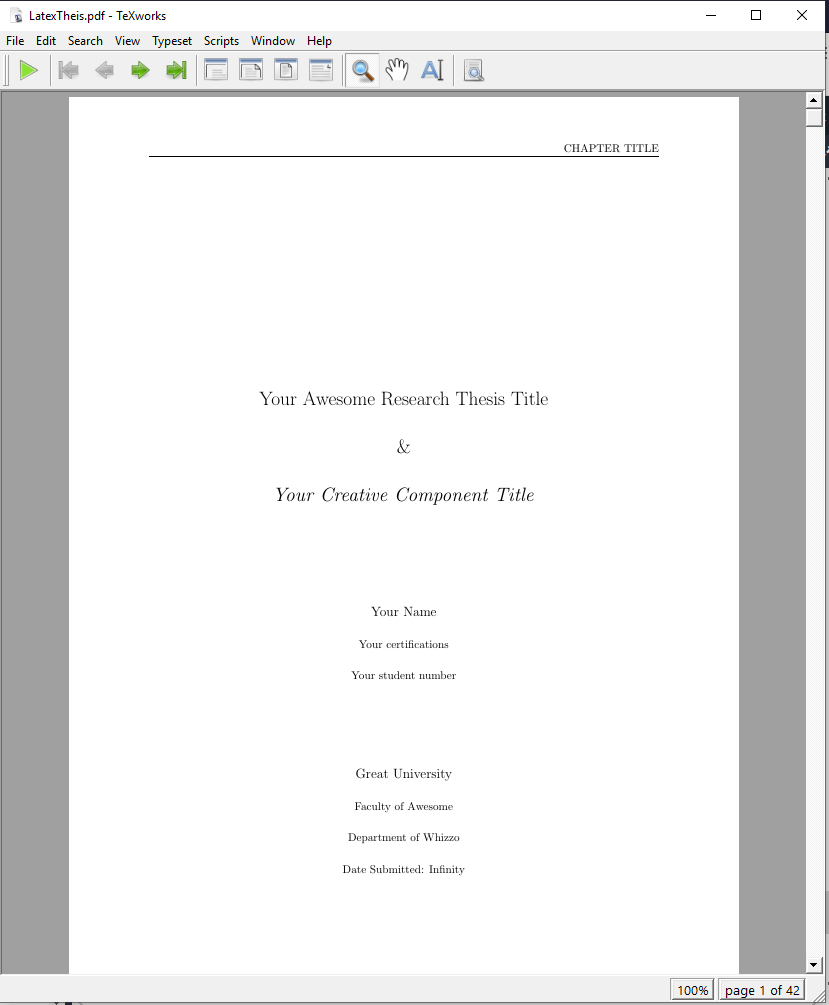
\includegraphics[width=350px]{images/tex010.PNG}

When you process the document TexWorks automatically saves the PDF when it displays the rendering.

It will save in the same location at the .tex file.

You now have a thesis  that is typeset appropriately for submission.

\section{Notes}

For some reason I have found I need to process the document twice to make the table of contents work. 

I have used a colleagues thesis as an example of the desired formatting for a creative thesis. This format may not be appropriate for your project.

\end{document}
